We use the wind tunnel datasets from Gamella et al. \citep{gamella2025causal}, featuring two controllable fans pushing air through a chamber, barometers measuring air pressure at various locations, and a hatch controlling an external opening. The tunnel is a chamber with two controllable fans that push air through it and barometers that measure air pressure at different locations. A hatch precisely controls the area of an additional opening to the outside (see Figure \ref{fig:causalchambers}).
\begin{figure}
    \centering
    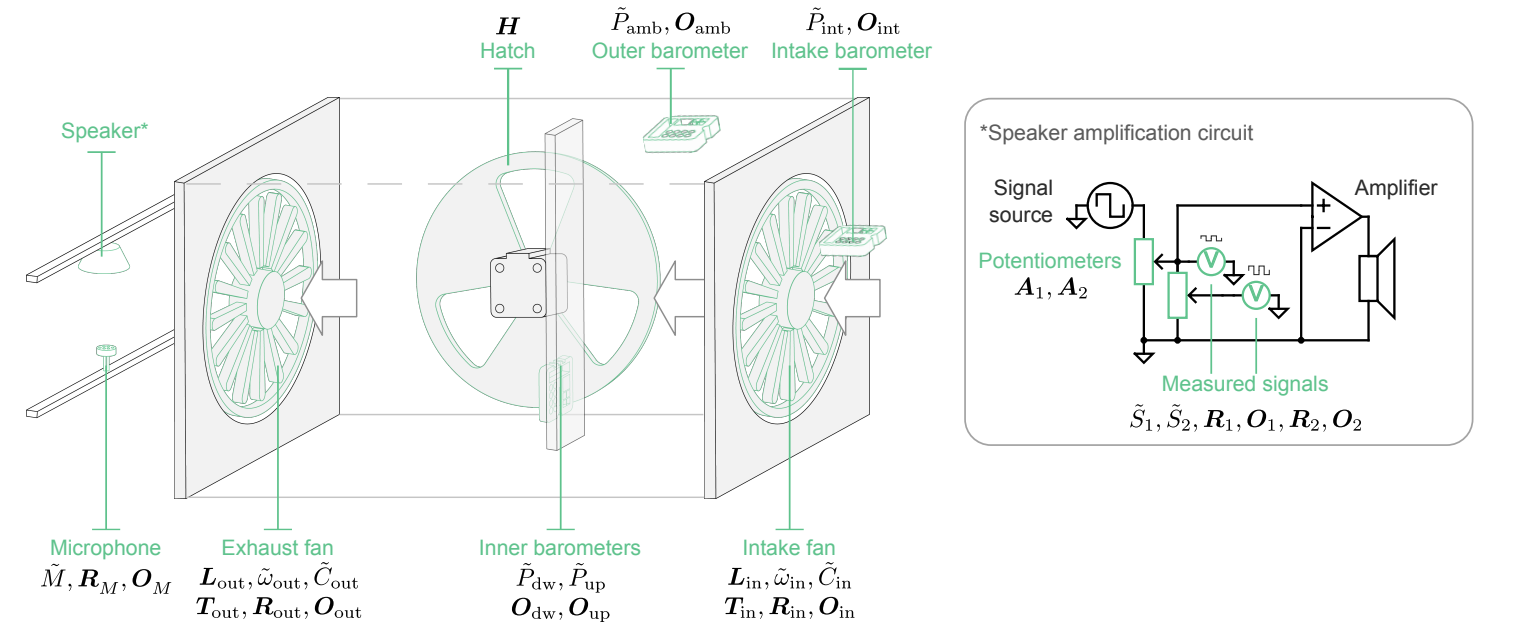
\includegraphics[width=0.9\linewidth]{figures/causalchambers.png}
    \caption{Figure taken from Gamella et al. \citep{gamella2025causal}. Diagrams of the wind tunel causal chamber and its main components, including the amplification circuit
that drives the speaker of the wind tunnel. The variables measured by
the chamber are displayed in black math print. Sensor measurements are denoted by a tilde. Manipulable variables, that is, actuators and sensor parameters, are shown in bold symbols. }
    \label{fig:causalchambers}
\end{figure}
The dataset comprises 16 variables: controllable load of the two fans $L_{in}, L_{out}$, their measurable speed $\left(\tilde{\omega}_{\text {in }}, \bar{\omega}_{\text {out }}\right)$, the current draw by the fans $\left(\tilde{C}_{\text {in }}, \tilde{C}_{\text {out }}\right)$ ( $\tilde{C}_{\text {in }}, \tilde{C}_{\text {out }}$ ), the resulting air pressure inside the chamber ( $\tilde{P}_{\text {dw }}, \tilde{P}_{\text {up }}$ ) or at its intake ( $\tilde{P}_{\text {int }}$ ), and the hatch $H$. In the circuit that drives the speaker, we can manipulate the potentiometers ( $A_1, A_2$ ) that control the amplification, monitoring the resulting signal at different points of the circuit $\left(\tilde{S}_1, \tilde{S}_2\right)$ and through the microphone output $(\tilde{M})$. $\tilde{\tilde{P}}_{\text {amb }}$ is the ambient pressure measure by the outer barometer. %["res_out", "osr_upwind", "v_out", "v_2", "v_in"],

We evaluate all the models on two regimes of 10,000 samples each: the first is observational, while the second involves soft interventions on five variables: 
\begin{itemize}
    \item $T_{\text {out }}$, the resolution of the tachometer timer that measures the elapsed time between successive revolutions of the fan. Choosing microseconds yields a higher resolution in the fan-speed measurement. Hence intervention on $T_{\text {out }}$ yields to a change on $\bar{\omega}_{\text {out }}$.
    \item $O_{\mathrm{up}}$ the oversampling rates when taking measurements of the current ( $\tilde{C}_{\text {in }}, \tilde{C}_{\text {out }}$ ), amplifier ( $\tilde{S}_1, \tilde{S}_2$ ) and microphone signals $(M)$, and of air pressure at the different barometers $\left(\tilde{P}_{\mathrm{up}}, \tilde{P}_{\mathrm{dw}}, \tilde{P}_{\mathrm{amb}}, \tilde{P}_{\mathrm{int}}\right)$.
    \item $R_{\text {in }}, R_{\text {out }}, R_2$ the reference voltages, in volts, of the sensors used to measure the current ( $\tilde{C}_{\text {in }}, \tilde{C}_{\text {out }}$ ), and amplifier ( $\tilde{S}_2$ ), respectively.
\end{itemize} 

For the training procedure, we start by a window of 6000 samples, which gives us three different initial regimes then FANTOM converges smoothly to the exact number of regimes $K=2$. We set our lag to 8 time lagged and we allow the presence of instantaneous parents. Regarding the parameters, we use a sparsity coefficient equal to 50, spline of 8 bins and MLPs of size 32.

We compare FANTOM to the baselines mentioned in the main text, with results in Table \ref{table2}. FANTOM is the only model that detects the regime with 99.9\% accuracy and outperforms all baselines on the graph learning task, achieving 38.5\% on F1 score. Notably, FANTOM surpasses all the models tailored for stationary MTS, even when they are given the ground-truth regime partitions. 

